%%%%%%%%%%%%%%%%%%%%%%%%%%%%%%%%%%%%%%%%%%%%%%%%%%%%%%%%%%%%%%%%%%%%%%%%%%%%%%%%%%%%%%%%%%%%%%%%%%%%%%%%%%%%%%%%%%%%%%%%%%%%%%%%%%%%%%%%
% This is just a template to use when submitting manuscripts to Frontiers, it is not mandatory to use frontiers.cls nor frontiers.tex  %
%%%%%%%%%%%%%%%%%%%%%%%%%%%%%%%%%%%%%%%%%%%%%%%%%%%%%%%%%%%%%%%%%%%%%%%%%%%%%%%%%%%%%%%%%%%%%%%%%%%%%%%%%%%%%%%%%%%%%%%%%%%%%%%%%%%%%%%%

\documentclass{frontiersSCNS} % for Science articles
%\documentclass{frontiersMED} % for Medicine articles

\usepackage{url}
\usepackage{tabularx}
\usepackage{lineno}
\usepackage{multirow}
\usepackage[english]{babel}
\usepackage{xcolor,colortbl}

\linenumbers

\newcommand{\R}{R}

\copyrightyear{}
\pubyear{}
%\onecolumn
%%% write here for which journal %%%
\def\journal{Neurosciences}
\def\DOI{}
\def\articleType{}
\def\citing{\color{darkgray}\cite}
\def\keyFont{\fontsize{6}{11}\helveticabold }
\def\firstAuthorLast{Duda {et~al}} %use et al only if is more than 1 author
\def\Authors{Jeffrey T. Duda\,$^{1,*}$, Philip A. Cook\,$^{1}$ and James C. Gee\,$^1$}
% Affiliations should be keyed to the author's name with superscript numbers and be listed as follows: Laboratory, Institute, Department, Organization, City, State abbreviation (USA, Canada, Australia), and Country (without detailed address information such as city zip codes or street names).
% If one of the authors has a change of address, list the new address below the correspondence details using a superscript symbol and use the same symbol to indicate the author in the author list.
\def\Address{$^{1}$Penn Image Computing and Science Laboratory, University of Pennsylvania, Department of Radiology, Philadelphia, PA, USA}
% The Corresponding Author should be marked with an asterisk
% Provide the exact contact address (this time including street name and city zip code) and email of the corresponding author
\def\corrAuthor{Jeffrey T. Duda}
\def\corrAddress{Penn Image Computing and Science Laboratory, University of Pennsylvania, Department of Radiology, 3600 Market Street, Suite 370, Philadelphia, PA, USA}
\def\corrEmail{jtduda@seas.upenn.edu}

% \color{FrontiersBlue} Is the blue color, used in the Journal name, in the title, and the names of the sections


\begin{document}
\onecolumn
\firstpage{1}

\title[Reproducibility of structural graph metrics]{Reproducibility of graph metrics of human brain structural networks}
\author[\firstAuthorLast ]{\Authors}
\address{}
\correspondance{}
\editor{}
\topic{Neuroinformatics with the Insight ToolKit}

\maketitle
\begin{abstract}

%\section{}
%As a primary goal, the abstract should render the general significance and conceptual advance of the work clearly accessible to a broad readership. References should not be cited in the abstract.
%See the Summary Table at \\ \url{http://www.frontiersin.org/}\texttt{\journal}\url{/authorguidelines} \\for abstract requirement and length according to article type.
% Abstract Max Length = 2000 characters 
Recent interest in human brain connectivity has led to the application of
graph theoretical analysis to human brain structural networks, in
particular white matter connectivity inferred from diffusion imaging
and fiber tractography. While these methods have been used to study a
variety of patient populations, there has been less examination of the
reproducibility of these methods. A number of tractography algorithms
exist and many of these are known to be sensitive to user-selected
parameters. The methods used to derive a connectivity matrix from
fiber tractography output may also influence the resulting graph
metrics. Here we examine how these algorithm and parameter choices
influence the reproducibility of proposed graph metrics on a publicly
available test-retest dataset consisting of 21 healthy adults. 
The dice coefficient is used to examine topological similarity
of constant density subgraphs both within and between subjects.
Seven graph metrics are examined here: mean clustering coefficient, 
characteristic path length, largest connected component size, assortativity,
global efficiency, local efficiency, and rich club coefficient. These reproducibility of
these network summary
measures is examined using the intraclass correlation coefficient
(ICC). Graph curves are created by treating the
graph metrics as functions of a parameter such as graph density.
 Functional data analysis techniques are used
to examine differences in graph measures that result from the choice
of fiber tracking algorithm. The graph metrics consistently showed
good levels of reproducibility as measured with ICC, with the exception of some instability at
low graph density levels. The global and local efficiency measures were 
the most robust to the choice of fiber tracking algorithm.

%A freely available data set, the Multi-Modal MRI Reproducibility Resource, will serve as the basis for this study. ANTs, based upon ITKv4, will be used for the registration and segmentation steps needed to align and label individual brains. Camino, an open-source toolkit, will be used for: DT reconstruction, fiber tracking, and the generation of structural connectivity matrices. An ITK module will be created to implement the graph analysis metrics.

\tiny
  \section{Keywords:} Structure, Tractography, Connectivity, Brain, Network, Reproducibility, Graph  %All article types: you may provide up to 8 keywords; at least 5 are mandatory.
\end{abstract}


% For Technology Reports the introduction should be succinct, with no subheadings.
\section{Introduction}
Combining magnetic resonance imaging (MRI) of the human brain with graph
theory analysis has emerged as a powerful approach to studying
large-scale networks of both structural and functional
connectivity. In the case of structural connectivity, the use of diffusion weighted MRI and
associated white matter fiber tractography methods provide the ability to identify
the long-range pathways that connect cortical regions and form a
network architecture~\citep{Basser2000,Lazar2003,Hagmann2003,Xue1999}. 
The use of graph theoretical analysis to study
the topology and structure of these large scale networks is an 
increasingly active topic of research \citep{Hagmann2008,Zalesky2010,Cheng2012,Bastiani2012,Irimia2012N,Sporns2011,Fornito2012}.
These methods have been used to examine the structural consequences of neurological disorders \citep{Xie2012,Guye2010,Martin2012}
as well as the relationship between structure and function \citep{Hagmann2008,Honey2009,Honey2007}. 

Previous studies examining the reproducibly of graph-based metrics in
functional networks have shown good levels of reproducibly in MEG
\citep{Deuker2009}, fMRI using BOLD contrast
\citep{Telesford2010,Braun2012,Schwarz2011,Liang2012,Weber2013} and
arterial spin labeling \citep{Weber2013}. A number of studies have also examined
reproducibly in structural networks, each focusing on various aspects
of the complex processing pipeline that is a prerequisite for these
measures. These have included studies of diffusion spectrum imaging
\citep{Cammoun2012,Bassett2011N} and high angular resolution diffusion
imaging \citep{Dennis2012}. Some studies have examined probabilistic
tractography \citep{Owen2013BC,Vaessen2010}. Diffusion tensor imaging (DTI) based studies using
deterministic tractography have included the examination of
tractography seed density \citep{Cheng2012N}, anatomic label density
\citep{Bassett2011N}, and studies examining a variety of network
measures \citep{Cheng2012N,Irimia2012N}. Further exploration of the reproducibility of
these graph metrics as it relates to their utility in longitudinal studies \citep{Telesford2013}.

In the paper we constrain our analysis to DTI-based deterministic fiber
tractography. Within this constraint, we examine multiple algorithms
for computing streamlines to examine their influence on the final graph metrics. A set of manually defined
cortical parcellations \citep{Klein2012} is used along with a more common template-based
parcellation scheme \citep{Tzourio-Mazoyer2002}. The intraclass correlation coefficient (ICC) is used to 
examine the reproducibility of network summary measures that results from combinations
of fiber tracking algorithm and anatomical label set. The dice coefficient provides a measure
of topographical similarity to examine the reproducibility of subgraphs extracted as a
function of graph density. Graph curves are constructed for a variety of metrics and functional data analysis is used
to examine how these metrics differ as a function of graph density or other parameters
that are specific to a given metric. We use freely
available data and software to create a framework that facilitates future extensions
that may examine additional aspects of the processing as well as the
comparison to, or addition of, multiple imaging modalities. 

%\begin{methods}
\section{Materials \& Methods}
% Materials and Methods: This section may be divided by subheadings. This section should contain sufficient detail so that when read in conjunction with cited references, all procedures can be repeated.

\subsection{Neuroimaging data}
The Multi-Modal MRI Reproducibility Resource \citep{Landman2011},
informally known as the Kirby dataset (\url{http://www.nitrc.org/projects/multimodal}), 
provides a publicly available test-retest data set consisting of 21
healthy control subjects (11 males). The mean
age is 31.76 $\pm$ 9.35 with a range of [22,61]. This data set provides a
multitude of MR image types, but here only the T1-weighted anatomical images and diffusion
tensor images are examined. The T1 images have a resolution of
$1.2 \times 1.0 \times 1.0 mm$. The distributed diffusion images have a resolution of
$0.828125 \times 0.828125 \times 2.2mm$. The diffusion data includes a single $b=0$
volume and 34 directional diffusion weighted images acquired with
$b=700 s/mm^2$. 

\subsection{Anatomical labeling}
A graph consists of nodes and the edges that connect those nodes. To construct a graph from a brain, a set of anatomical labels
are used to define the nodes of the graph. To determine if manually defined cortical labels would provide an inherent advantage in
reproducibility we used of the Mindboggle dataset which provides a set of manually drawn cortical regions (DKT31) 
along with a skull-stripped image for a single time point for each subject in the Kirby data set \citep{Klein2012}. 
To utilize these labels in network creation we performed an intra subject registration between each subject's two T1 images. 
A brain mask was created from the provided skull-stripped T1 image by thresholding and a morphological closing. This mask
was warped into the unlabeled T1 image space and used to create a skull-stripped image. For each time, a transformation was found
between the skull-stripped T1 image and the b=0 image, acquired as part of the DTI acquisition. In all subjects, the manually defined
labels were propagated into the DTI space for both time points using the appropriate composed transform. 

One of the most common label sets used in studies of both functional and structural
connectivity is the AAL label set \citep{Tzourio-Mazoyer2002} which is a template based label set. An existing multivariate template had 
been created from the Kirby dataset using the \texttt{antsMultivariateTemplateConstruction.sh} tool, part of the 
Advanced Normalization Tools (ANTs) software package \citep{ANTS}. The \texttt{antsRegistration} tool was used to find
a deformable mapping between the T1 template image distributed with the AAL label and the population specific template
created from the Kirby data.  In order to transform these labels into each 
subject's DTI space, it was necessary to find a transform from the template to each subject's T1 and from T1 to DTI within 
each subject. For the template-to-T1 transform, the \texttt{antsCorticalThickness.sh} tool was used. This software first applied a bias
correction using the N4 algorithm \citep{Tustison2010}. Next a registration based skull stripping was performed to provide
a cerebrum mask of the T1 image. This was followed by a final cerebrum-only registration to the template. These transforms were
composed with the T1-to-DTI transforms, providing a single transform that was used to warp the the AAL labels into DTI space using nearest neighbor interpolation. Labels of structures outside of the cerebrum were removed.
Many AAL labels include both gray and white matter, here the labels were masked to only include voxels 
that were identified as cortical gray matter by the DKT31 labels described in the previous section. 
The AAL labels for deep gray structures (e.g.\ thalamus) were not masked but used in their entirety. Both label sets are illustrated
in figure \ref{fig:labels}, while the entire processing scheme is
illustrated in figure \ref{fig:scheme}. The availability of the
processing scripts is intended to provide a framework that allows for
convenient exploration of alternate anatomical labels, such as the
anatomical parcellations that may be obtained via FreeSurfer
(\url{http://surfer.nmr.mgh.harvard.edu}) or the UCLA Multimodal
Connectivity Package
(\url{http://ccn.ucla.edu/wiki/index.php/UCLA_Multimodal_Connectivity_Package}),
both of which have been used in previous graph-theory based examinations of structural connectivity based on diffusion-weighted imaging.

\begin{figure*}
\begin{center}
\renewcommand{\tabcolsep}{0pt}
\renewcommand\arraystretch{0}
\begin{tabular}{ccccccc}
%\includegraphics[width=0.14\linewidth]{figures/aal120.png} & 
%\includegraphics[width=0.14\linewidth]{figures/aal130.png} & 
%\includegraphics[width=0.14\linewidth]{figures/aal140.png} & 
%\includegraphics[width=0.14\linewidth]{figures/aal150.png} & 
%\includegraphics[width=0.14\linewidth]{figures/aal160.png} & 
%\includegraphics[width=0.14\linewidth]{figures/aal170.png} & 
%\includegraphics[width=0.14\linewidth]{figures/aal180.png} \\
%\includegraphics[width=0.14\linewidth]{figures/dkt120.png} & 
%\includegraphics[width=0.14\linewidth]{figures/dkt130.png} & 
%\includegraphics[width=0.14\linewidth]{figures/dkt140.png} & 
%\includegraphics[width=0.14\linewidth]{figures/dkt150.png} & 
%\includegraphics[width=0.14\linewidth]{figures/dkt160.png} & 
%\includegraphics[width=0.14\linewidth]{figures/dkt170.png} & 
%\includegraphics[width=0.14\linewidth]{figures/dkt180.png}
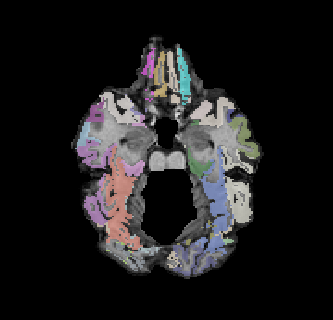
\includegraphics[width=0.14\linewidth]{figures/aal_125_masked.png} & 
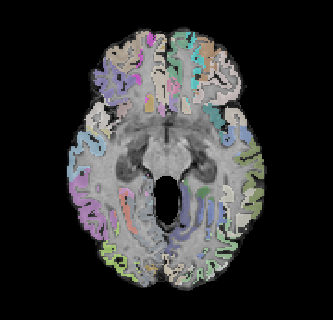
\includegraphics[width=0.14\linewidth]{figures/aal_135_masked.png} & 
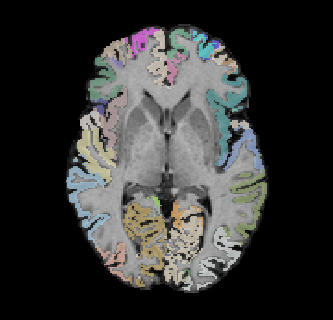
\includegraphics[width=0.14\linewidth]{figures/aal_145_masked.png} & 
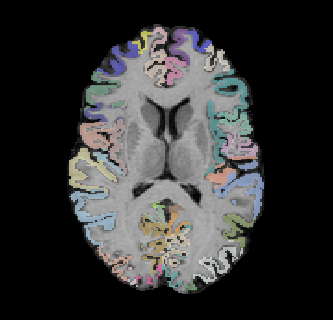
\includegraphics[width=0.14\linewidth]{figures/aal_155_masked.png} & 
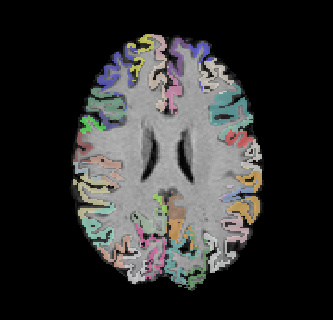
\includegraphics[width=0.14\linewidth]{figures/aal_165_masked.png} & 
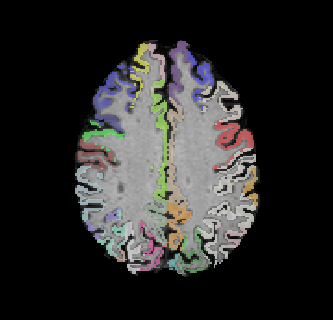
\includegraphics[width=0.14\linewidth]{figures/aal_175_masked.png} & 
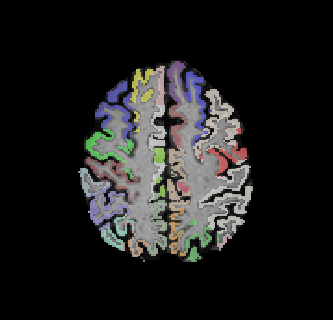
\includegraphics[width=0.14\linewidth]{figures/aal_185_masked.png} \\
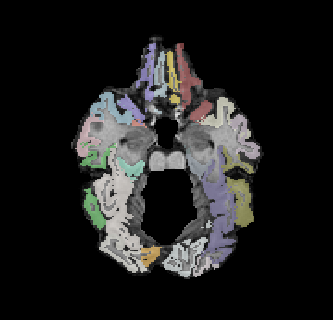
\includegraphics[width=0.14\linewidth]{figures/dkt_125_masked.png} & 
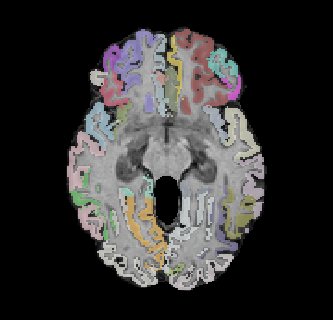
\includegraphics[width=0.14\linewidth]{figures/dkt_135_masked.png} & 
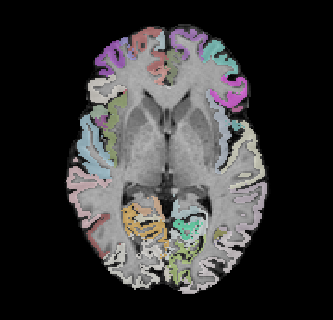
\includegraphics[width=0.14\linewidth]{figures/dkt_145_masked.png} & 
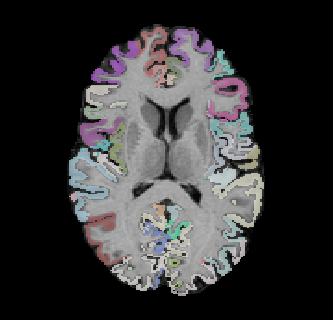
\includegraphics[width=0.14\linewidth]{figures/dkt_155_masked.png} & 
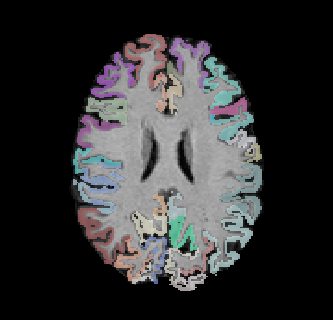
\includegraphics[width=0.14\linewidth]{figures/dkt_165_masked.png} & 
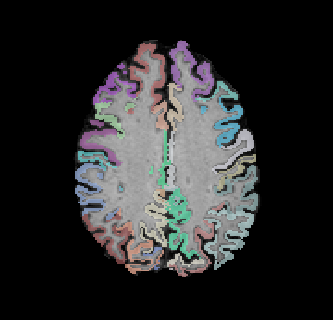
\includegraphics[width=0.14\linewidth]{figures/dkt_175_masked.png} & 
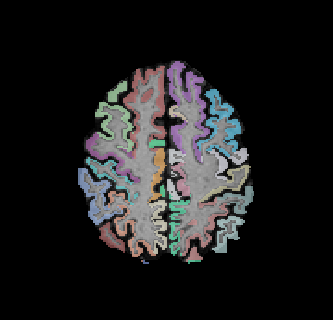
\includegraphics[width=0.14\linewidth]{figures/dkt_185_masked.png}
\end{tabular}
\caption{Two sets of anatomical labels are used to define the
  networks. The template based AAL labels (top) and The DKT31 manually
  defied labels that are provided via Mindboggle (bottom). The AAL
  labels have been masked to only include gray matter}
\label{fig:labels}
\end{center}
\end{figure*}
%\textbf{Figure 1.}{Two sets of anatomical labels are used to define the networks. The template based AAL labels (top) and The DKT31 manually defined labels that are provided via Mindboggle (bottom). }\label{fig:01}

\begin{figure*}
\begin{center}
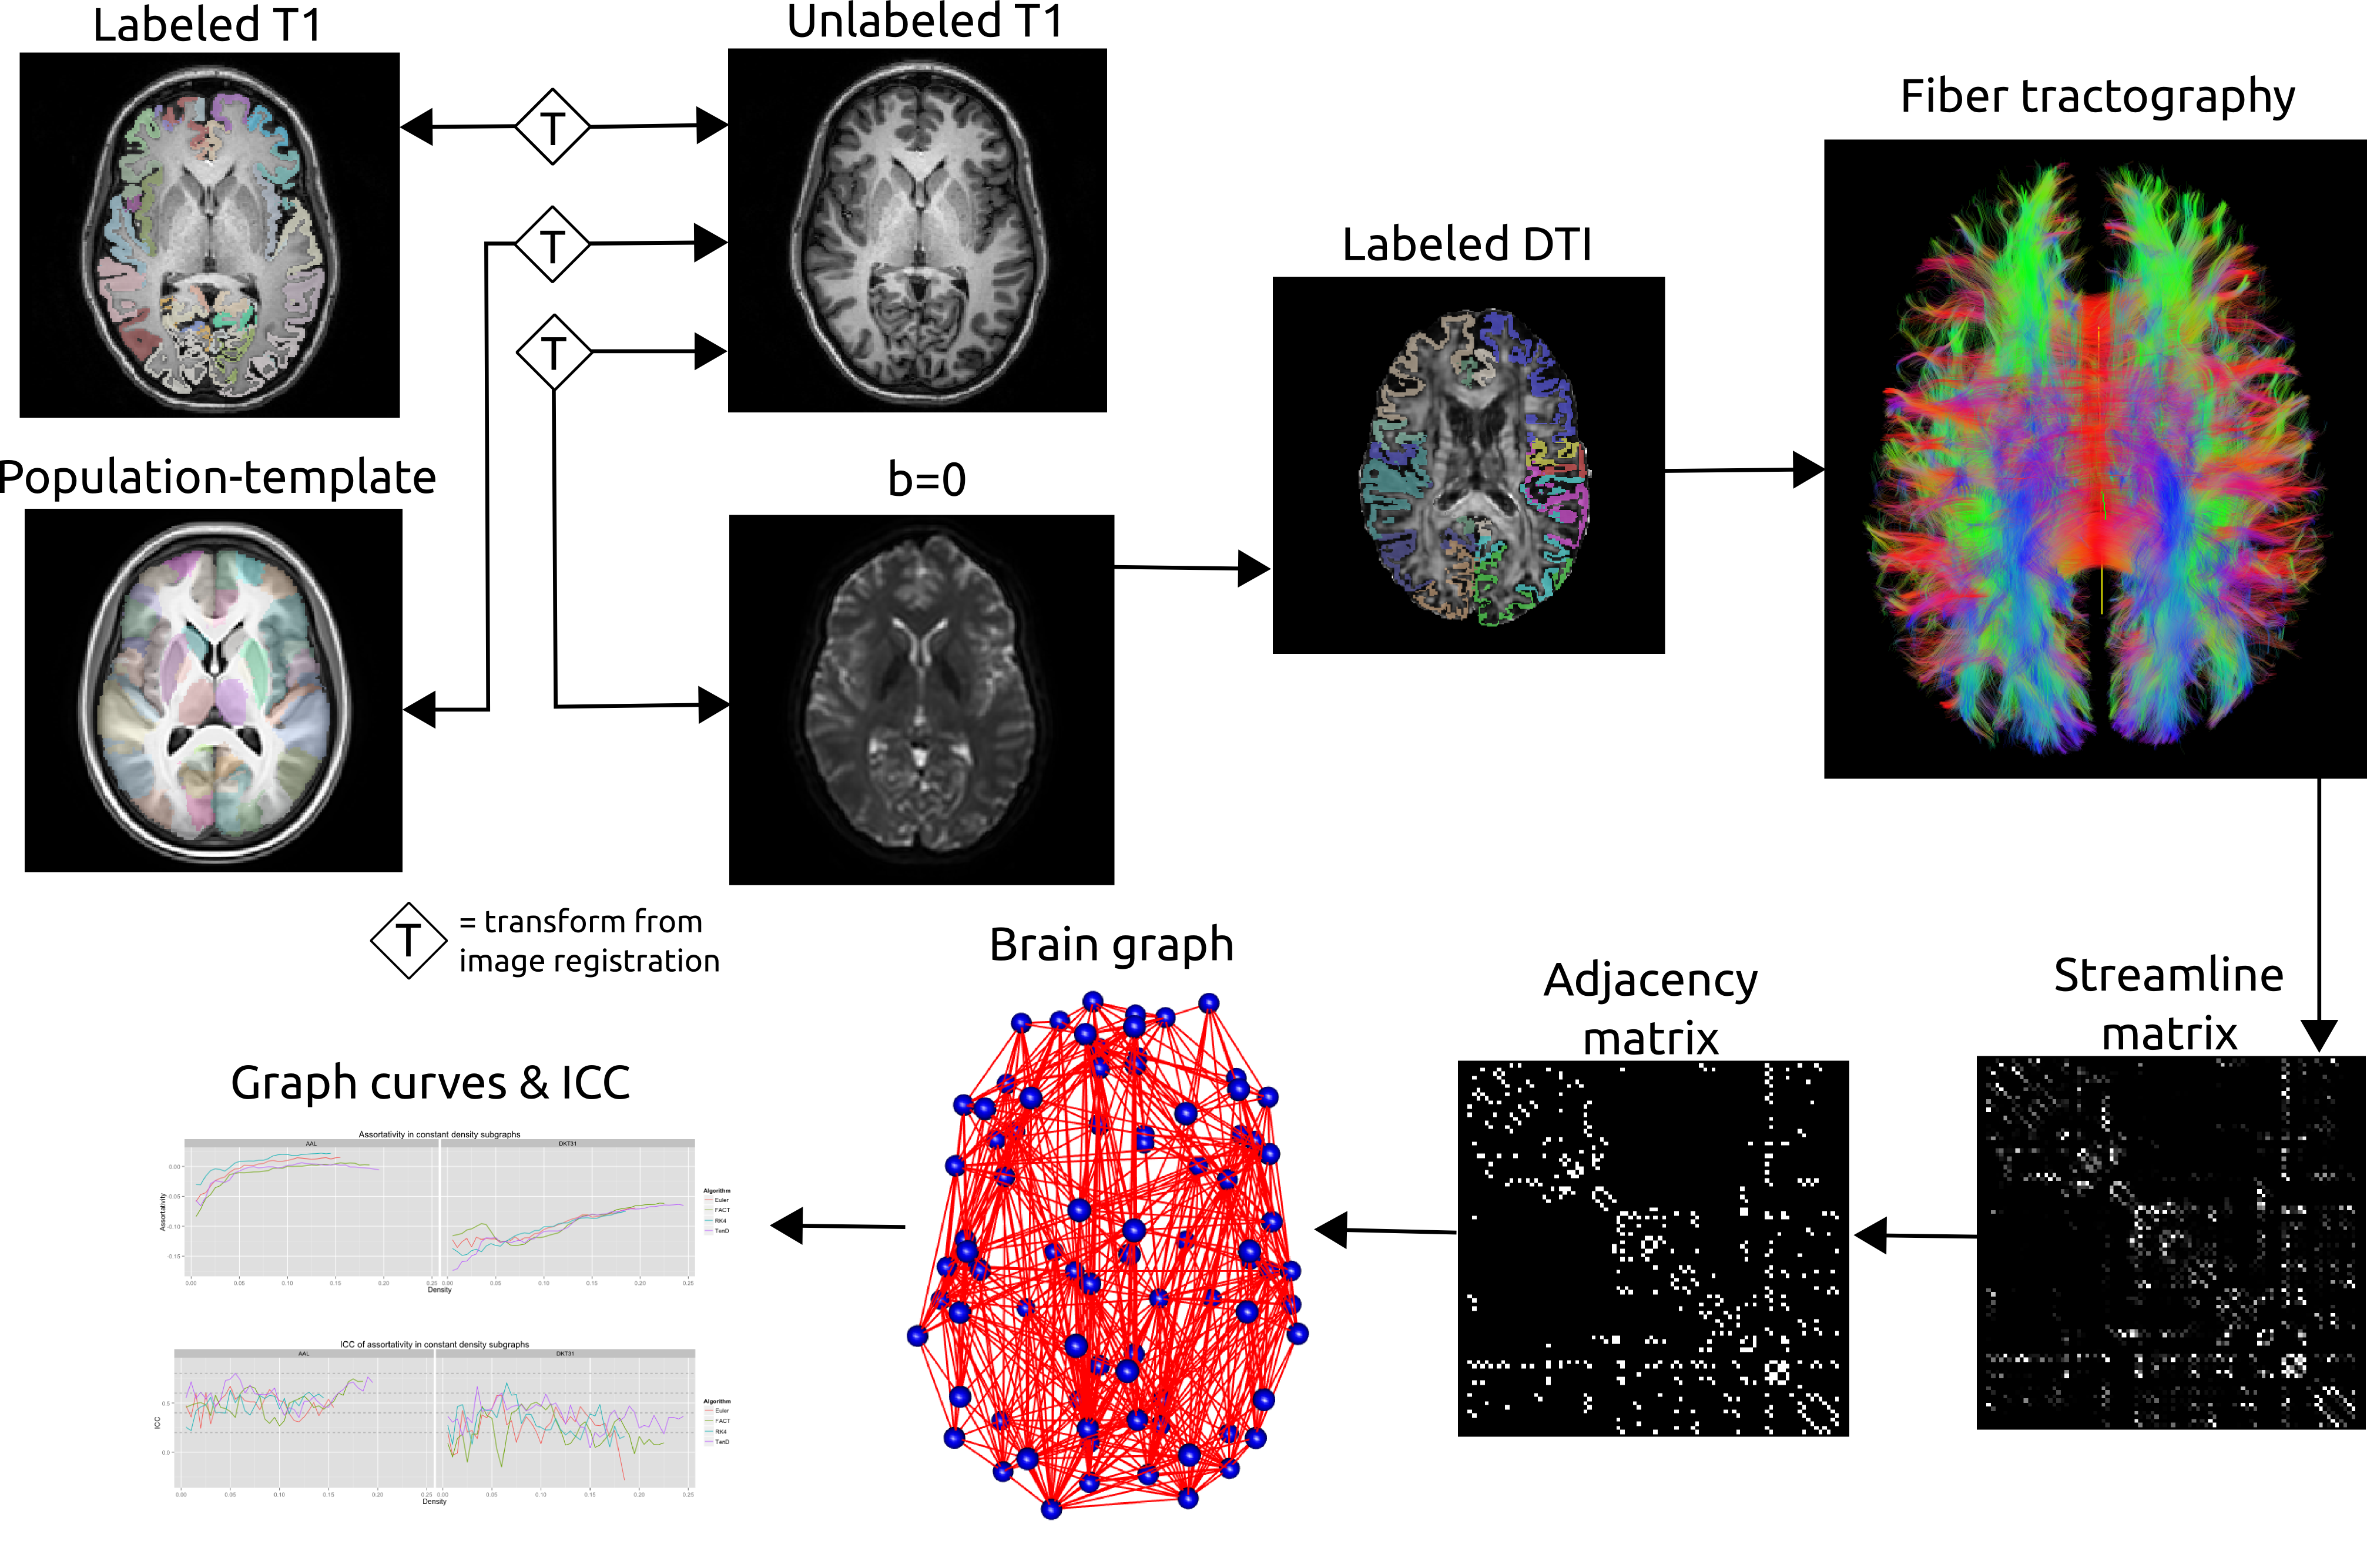
\includegraphics[width=\linewidth]{figures/flow.png} 
\caption{Schematic of the network processing scheme. Image registration is used to find transformations between the T1 image and: the T1 image for that subject's other time point; the population template; the b=0 image acquired as part of the DTI acquisition. Labels are transformed into the DTI space where fiber tractography is performed. A matrix is created that records the number of streamline connecting each pair of labeled regions. This matrix is thresholded as constant density to create an adjacency matrix which defines connections in a brain graph. Graph curves are generate by calculating network summary measures over a range of density values and ICC plots are used to examine the reproducibility of the metrics.}
\label{fig:scheme}
\end{center}
\end{figure*}
%\textbf{Figure 2.}{Schematic of the network processing scheme. Image registration is used to find transformations between the T1 image and: the T1 image for that subject's other time point; the population template; the b=0 image acquired as part of the DTI acquisition. Labels are transformed into the DTI space where fiber tractography is performed. A matrix is created that records the number of streamline connecting each pair of labeled regions. This matrix is thresholded as constant density to create an adjacency matrix which defines connections in a brain graph. Graph curves are generate by calculating network summary measures over a range of density values and ICC plots are used to examine the reproducibility of the metrics.}\label{fig:02}

\subsection{Diffusion data preprocessing}
The Camino toolkit \citep{Cook2006} was used to calculate diffusion tensor images via a
weighted linear fitting \citep{Basser1994c,Salvador2005b}, and was 
used for subsequent deterministic tractography. The brain masks defined
in T1 space were warped into DTI space and used to prevent tracking outside the brain. 
Fractional anisotropy (FA) images were calculated and a
tractography seed-map was created to include all voxels in the cerebrum with an FA of at
least 0.2. 

One of the primary differences among the various approaches to
deterministic tractography is the algorithm used to determine the
direction that a streamline should proceed from a given point. Here we
examine four different approaches:

\begin{enumerate}
\item Fiber Assignment by Continuous Tracking (FACT) - The primary
  direction of diffusion (PDD) is followed until the streamline enters
  a new voxel \citep{Xue1999}.
\item Euler -  The PDD is followed for a constant step size \citep{Basser2000}.
\item Rourth-order Runge-Kutta (RK4) - The direction of the step is determined
 by taking and averaging a weighted series of partial steps \citep{Basser2000}.
\item Tensor Deflection (TEND) - The local fiber trajectory is a function of the previous
direction and the local diffusion tensor \citep{Lazar2003}
\end{enumerate}

Shared parameters used in the fiber tracking were held constant as follows
\begin{enumerate}
\item Streamlines were terminated if curvature of more than 90 degrees over 5 steps was detected. 
\item Streamlines were terminated if an FA value of less of 0.2 was encountered. 
\item A step size of 0.5mm was used. 
\item Linear interpolation of the primary direction of diffusion was used for Euler and RK4. 
\end{enumerate}

Figure \ref{fig:tracts} illustates the fiber tracts for all methods for a single subject. The script used to generate these streamlines,
\texttt{deterministic\textunderscore mmrr21.pl}, is available as part of the git
repository that contains all of the processing scripts for the work
presented here (\url{https://github.com/jeffduda/StructConnRepro}). Relatively small
changes to this script would allows users to explore additional
deterministic tractograpy methods as well as probabilistic methods
which are also available in the Camino toolkit.

\begin{figure*}
\begin{center}
\renewcommand{\tabcolsep}{0pt}
\renewcommand\arraystretch{0}
\begin{tabular}{ccccccc}
FACT & Euler & RK4 & TenD \\
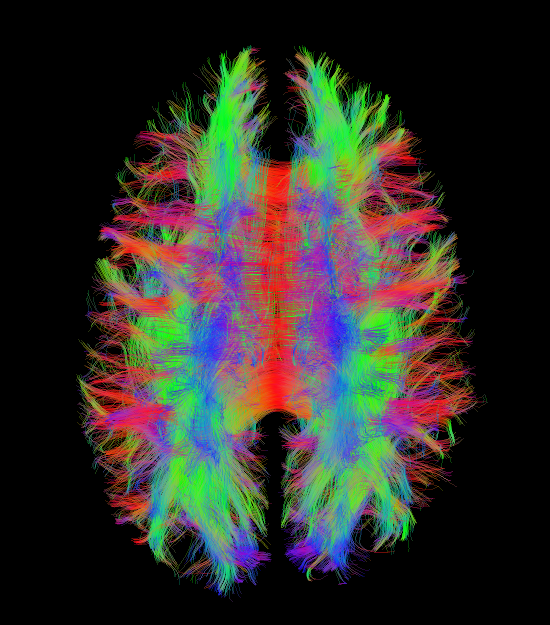
\includegraphics[width=0.25\linewidth]{figures/113_30_fact.png} & 
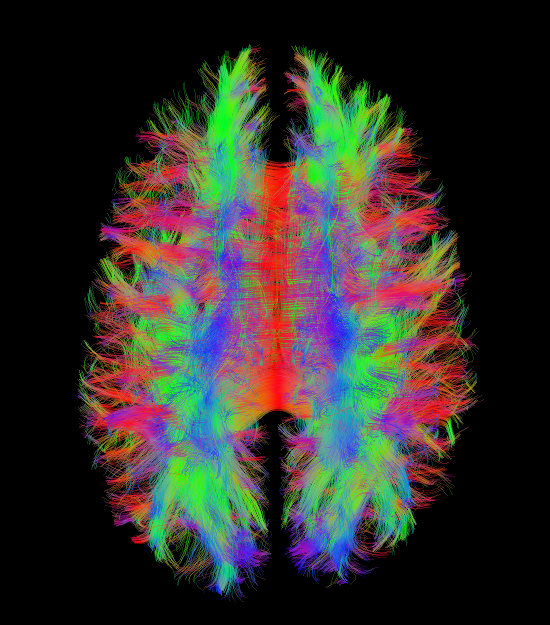
\includegraphics[width=0.25\linewidth]{figures/113_30_euler.png} & 
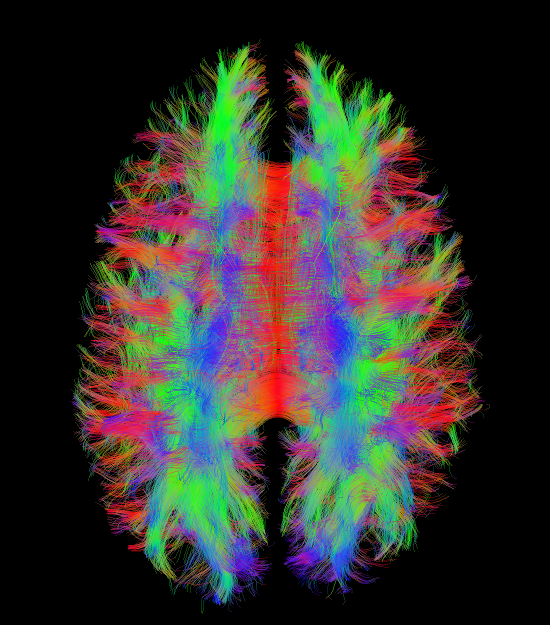
\includegraphics[width=0.25\linewidth]{figures/113_30_rk4.png} & 
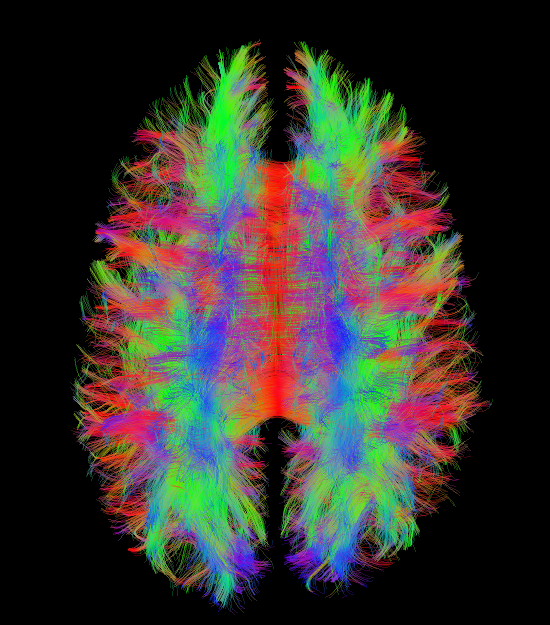
\includegraphics[width=0.25\linewidth]{figures/113_30_tend.png} \\
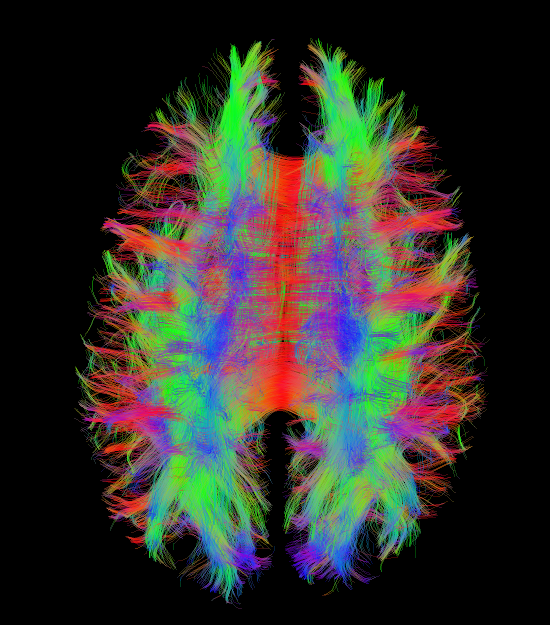
\includegraphics[width=0.25\linewidth]{figures/113_33_fact.png} & 
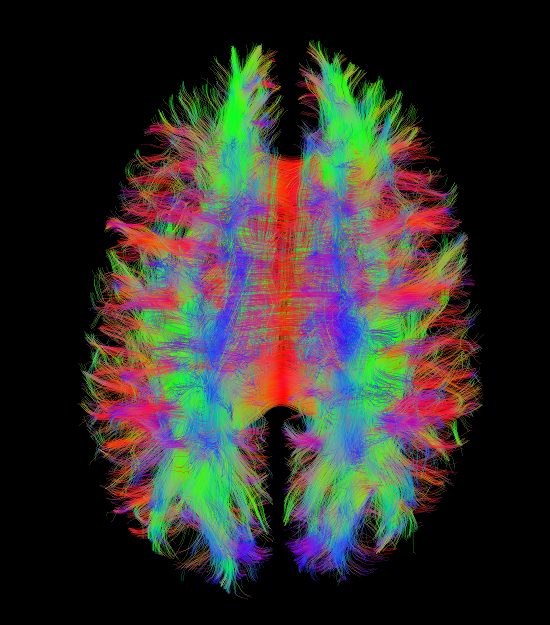
\includegraphics[width=0.25\linewidth]{figures/113_33_euler.png} & 
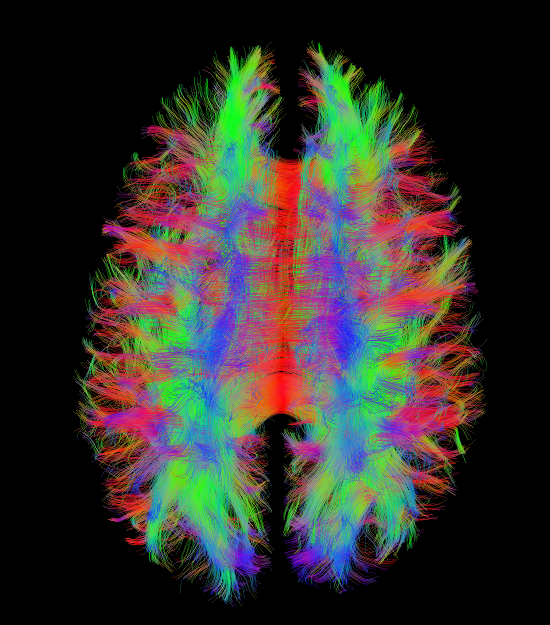
\includegraphics[width=0.25\linewidth]{figures/113_33_rk4.png} & 
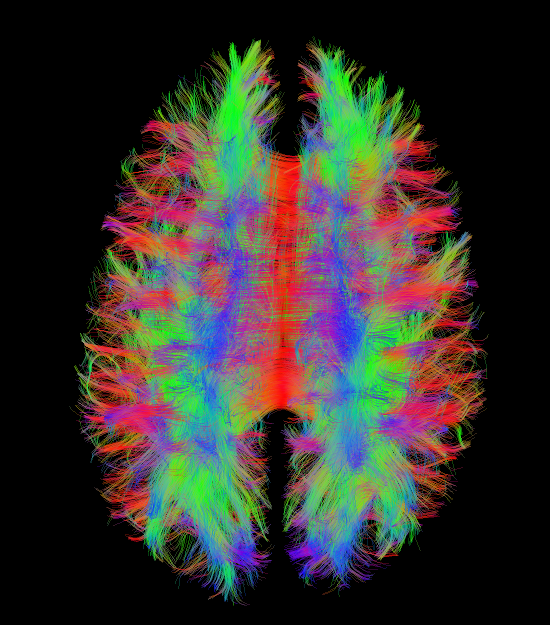
\includegraphics[width=0.25\linewidth]{figures/113_33_tend.png} \\
\end{tabular}
\caption{Fiber tracts generated using each method are illustrated for both time points in a single subjects. For visualization, tract sets are sampled to display 5\% of the tracts at 25\% opacity. Tract points are colored to illustrate local streamline direction.}
\label{fig:tracts}
\end{center}
\end{figure*}

%Additionally we examine the weighting parameters used in the TEND
%algorithm

\subsection{Graph generation}
While the nodes of a graph were defined using anatomical labels, the edges of the graph were defined by using
fiber tractography to identify white matter pathways that connect brain regions. 
For a given set of streamlines, the \texttt{connmat} tool provided by  the Camino toolkit was used to generate
a connectivity matrix that records how many streamlines connect each pair of
regions in a given set of target regions. This program starts at the seed point for a streamline and proceeds outward in each
direction to determines the two target regions encountered. Only streamlines that connect two unique regions are retained and
a given streamline may be only be counted as connecting a single pair of target regions. Fiber tractography does not provide a measure
of directionality (i.e.\ neither node can be considered a starting point or ending point) so the resulting matrices resulting in undirected graphs.

Graph are often compared by first ensuring that they have the same density \citep{Achard2006,Bassett2006}, where density for an undirected graph is defined as:
$$D(G) = \frac{\|E(G)\|}{( \|N(G)\| (\|N(G)\|-1) )} $$
where $N(G)$ is the set of all nodes in graph $G$ and $E(G)$ is the set of all edges in $G$. The number of nodes in the graph and the desired density determine the number of edges that the graph should contain. Edges of higher weights are given priority and lower weighted edges are removed to obtain the desired density level. The weights of the remaining edges are then set to 1 for a final binarized graph. This cumulative thresholding provides a normalized method for comparing network measures as it results in the comparison of graphs with an equal percentage of significant connections. Graphs are typically compared over a range of density levels.  Here, we only directly compare measures obtained from graphs with an equal number of nodes and thus an equal number of edges after density thresholding.

\subsection{Network metrics}
A large number of graph metrics are available for quantifying properties of binary, undirected networks \citep{Rubinov2010}. Here we examine a number that 
are common in current literature: largest connected component size \citep{Bassett2011N}, assortativity\citep{Newman2006a,Bassett2008}, clustering coefficient \citep{Watts1998}, characteristic path length\citep{Watts1998}, global and local efficiency \citep{Latora2001}, and rich club coefficient\citep{Collin2013}. An ITK module named Petiole (\url{https://github.com/jeffduda/Petiole}) was created to calculate these network measures from 2D connectivity
matrices. This module incorporates and extends an existing implementation of a graph class \citep{Tustison2008} and provides ITK functions for a variety of graph metrics while using the matlab-based Brain Connectivity Toolkit \citep{Rubinov2010} for algorithmic guidance. While many of these metrics include implementations for weighted graphs and/or directed graphs, here we focus on their application to unweighted, undirected graphs. Summaries and equations for these metrics are provided here:

\emph{Size of Largest Connected Component}.  A connected component of a graph is a subset of the graph, $G_{i}$, where there exists a path between all pairs of nodes and for which no path exist to additional nodes in $G$. The largest connected component is the $G_{i}$ with the greatest number of nodes, $\|N(G_{i}\|$. This measure relates to the global level of connectivity within a subject's brain network~\cite{Bassett2011N}.

\emph{Assortativity}. The degree of a node is the number of neighboring nodes that it connects to (i.e.\ shares an edge with). Assortativity measures how preferentially nodes of similar degree connect to one another \citep{Newman2006a} and is defined as:
$$A =  \frac{ \frac{1}{E} \sum_{i}{j_i k_i} - [ \frac{1}{E} \sum_{i}{ \frac{1}{2} (j_i + k_i)} ]^2 }{ \frac{1}{E} \sum_{i}{ \frac{1}{2}( j_{i}^{2} + k_{i}^{2} ) } - [ \frac{1}{E} \sum_{i}{ \frac{1}{2} (j_i + k_i)} ]^2  } $$
where $j_i,k_i$ are the degrees of the nodes connected by edge $i$ and $E = \|E(G)\|$. High assortativity suggests higher network resilience, making a network less vulnerable to attack \citep{Newman2002}.

\emph{Clustering Coefficient}. This measure quantifies how likely is that two nodes with a common neighbor are connected to one another ~\citep{Watts1998}. Here we calculate the clustering coefficient at each node and calculate the mean over all nodes in the network for our final network summary measure. The clustering coefficient at node $i$ is given by:
$$C_i = \frac{e_i}{\|K_i\| ( \|K_i\| -1 )}$$
where $K_i$ is the set of all nodes that share an edge with $i$ and $e_i$ is the set of all edges that connect nodes in $K_i$.

\emph{Characteristic Path Length}. The pathlength, $L_{ij}$, that connects two nodes, $i$ and $j$, is defined as the minimum number of edges that must be traversed to travel from $i$ to $j$ \citep{Dijkstra1959}. The characteristic path length is the average pathlength over all possible pairs of connections in a graph. In an undirected graph this is:
$$L = \frac{1}{\|N(G)\|(\|N(G)\|-1)} \sum_{ij \in G, i \neq j}{L_{ij}}$$
This measure is only defined for fully connected graphs. Here, we apply the density thresholding first and then extract the largest connected component in order to calculate the characteristic path length.

\emph{Global Efficiency}. This measure is related to the
characteristic path length, in that it attempts to quantify the mean
efficiency between any two nodes in the graph. Unlike the
characteristic path length, this metric is defined for both connected and unconnected graphs \citep{Latora2001}.
$$F_{glob} = \frac{1}{\|N(G)\|(\|N(G)\|-1)} \sum_{i \neq j \in G}{1/L_{ij}}$$

\emph{Local Efficiency}. This metric relates to fault tolerance and examines efficiency between neighbors on a node $i$, if that node were removed from the graph \citep{Latora2001}.
$$F_{loc} = \frac{1}{\|N(G)\|} \sum_{i \in n}{F(G_i)}$$
where $G_i$ is the subgraph of $G$ that results from removing node $i$.

\emph{Rich Club Coefficient}
This measures quantifies how preferentially the high-degree nodes (i.e. rich nodes)  in a graph connect to other high-degree nodes \citep{Colizza2006}.
$$ R(G,k) = \frac{ \|E(G,k)\| }{ \|N(G,k)\| ( \|N(G,k)\|-1 ) } $$
where $N(G,k)$ is the set of nodes of degree k or higher and $E(G,k)$ is the set of edges connecting two nodes in $N(G,k)$.


\subsection{Graph curves}
The metrics listed above are all applied to thresholded binary graphs. As discussed earlier, this binary graph result from thresholding at a constant density. These metrics may then be treated as functional curves of metric vs. graph density. By doing this, we are able to compare binary graphs in a way that incorporates the continuous structure of the original connectivity matrices. The rich club coefficient however is dependent upon two parameters, the graph density and, $k$, the degree threshold used to determined what constitutes a rich-node. For this metric we threshold at the highest density common to all graphs and explore how the value changes with $k$. For all other metrics, we examine their curves as a function of graph density. 

\subsection{Statistical analysis}
Before examining how the graph metrics change with density it is necessary to examine the maximum density of the graphs to determine the range over which graphs may be compared. Additionally, it is interesting to examine the topological similarity in the thresholded graphs. This is done using the dice coefficient which measures similarity between two graphs as:
$$Dice(x,y) = \frac{ 2 \| E(x) \cap E(y) \| }{ \|E(x) \| + \| E(y) |\ }$$
where edges are considered equal if they connect the same two
nodes. This is equivalent to treating each connectivity matrix as
a binarized 2D image and using the Dice metric to measure overlap. The mean intra- and inter-subject topological similarity 
was computed over a range of densities for each combination of tracking algorithm and anatomical label sets. This allows us to 
examine the reproducibility of within-subject topography compared to between subject topography. This metric is limited to lie in the range $[0,1]$ and can be interpreted as a measure of degree of overlap between graphs. This provides a stricter metric than measuring overlap between sets of nodes as complete node-overlap is a necessary but incomplete condition for complete edge-overlap.

Graph curves are used to examine the reproducibility of the graph metrics as a function of an independent parameter, typically graph density. At each point along the curve, reproducibility of the metric is quantified using the ICC:
$$ICC = \frac{\sigma_{bs}^{2}}{\sigma_{bs}^{2} + \sigma_{ws}^{2}} $$
where $\sigma_{bs}^{2}$ is the between-subject variance and $\sigma_{ws}^{2}$ is the within subject variance. The 'ICC' package for  \R{} is used for this calculation. The ICC is plotted along with the mean graph metrics for each combination of algorithm and label set. At points where little to no variance exists in a graph metric, the ICC is not calculated as it becomes unstable under those conditions. The following guidelines may be used to interpret ICC values: ICC $<$ 0.2 'poor agreement'; 0.21 - 0.40 'fair agreement'; 0.41-0.60 moderate agreement; 0.61-0.80 'strong agreement'; ICC $>$ 0.8 'near perfect agrement \citep{Telesford2010,Montgomery2002}. Dashed lines indicating the boundaries of these categories have been included on all ICC plots to aid interpretation.

To identify group diferences that result from fiber tracking algorithm we incorporated methods from functional data analysis (FDA) which treats each curve as a function. For each group, the set of all curves were averaged to create a single mean curve.  While there are a variety of methods for computing the difference between two curves, here we chose the simplest method, the non-parametric permutation test. Each mean curve was treated a function and the area between the group mean curves was found. Individual group assignments were then permuted using random sampling without replacement and then  used to calculate mean curves . The area between the random-group mean curves was calculated. This was performed iteratively (i=10000). We recorded, x, the number of times area between the mean curves from the randomly assigned groups is larger than the area between the true group mean curves. The p-value for the true group difference is then defined as $x/i$. We report these differences for between-algorithm curves as they derive from graph of equal size, but do compare curves that derive from different anatomical label sets.

%\textbf{Figure 1.}{ Enter the caption for your figure here.  Repeat as  necessary for each of your figures.}\label{fig:01}% Don't add the figures in the LaTeX files, please upload them when submitting the article. Frontiers will add the figures at the end of the provisional pdf.

%\end{methods}

\section{Results}
%Results: This section may be divided by subheadings. Footnotes should not be used and have to be transferred into the main text
\subsection{Network density}
Maximal densities for connectivity matrices across all tracking
algorithm ranged from 0.17 to 0.30 for the AAL labels and from 0.20 to
0.41 for DKT31. Maximal densities in the DTK31 data was generally
higher than in the AAL as illustrated in figure
\ref{fig:density}. Both label sets had the same lowest-to-highest
ordering of mean maximal density within algorithms: RK4 $<$ Euler $<$
FACT $<$ TEND.


\begin{figure}
\begin{center}
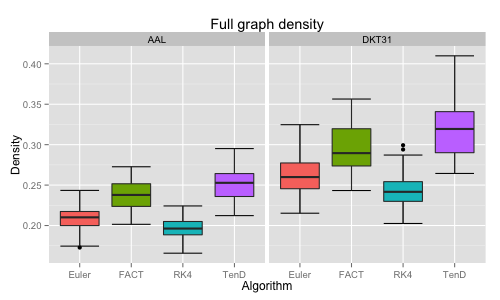
\includegraphics[width=0.5\linewidth]{figures/density_plot.png} 
\caption{Boxplots illustrating the density values for unthresholded connectivity matrices for all subjects and all time points, grouped by fiber tracking algorithm (Euler,FACT,RK4,TEND) and anatomical label set (AAL,DKT31).}
\label{fig:density}
\end{center}
\end{figure}

\subsection{Network topology}
Dice coefficients for intra-subject similarity ranged from 0.70 to
0.81 for the AAL labels and from 0.59 to 0.82 for the DTK31
labels. Inter-subject similarity ranged from 0.51 to 0.71 for AAL
labels and from 0.32 to 0.71 for the DTK31 labels. For all
algorithm-label pairings, intra-subject overlap was greater than
inter-subject overlap across the range of densities as illustrated in
figure \ref{fig:dice}. Permutation testing of intra-subject dice
vs. density curves did not reveal any significant differences between
algorithms for either label set. However, a number of differences were
found in the inter-subject comparions. The resulting p-values are
listed in table \ref{tab:dicep}. 

\begin{figure}
\begin{center}
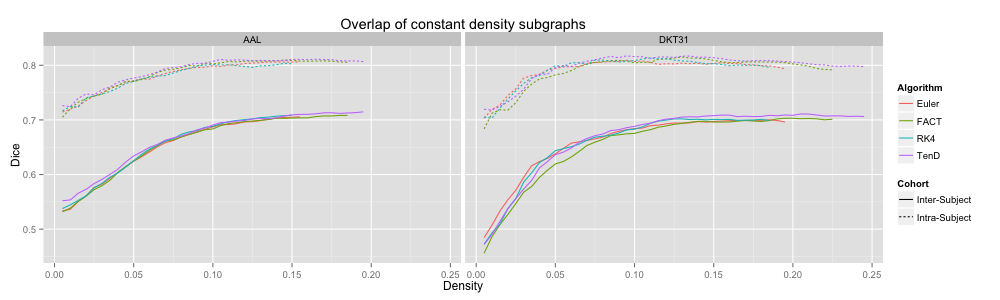
\includegraphics[width=0.5\linewidth]{figures/dice_overlap_plot.png} 
\caption{Connectivity matrices were thresholded over a range of density values. At each density level, consistency of network topography was estimated by calculating the mean dice overlap for both intra subject and intersubject pairs.}
\label{fig:dice}
\end{center}
\end{figure}

%\begin{table}[!t]
%\processtable{Dice p-values.\label{tab:dicep}}
%{\begin{tabular}{l | llll}
%\midrule
 %        & Euler    & FACT     & RK4        & TEND      \\ \midrule
%Euler  &            & 0.9555  & 0.9864    & 0.6549   \\
%FACT & 0.7770 &              & 0.7970  & 0.9524     \\
%RK4   & 0.2675 & 0.2586   &               & 0.5358    \\
%TEND & 0.0351 & 0.0351*  & 0.1335    &                 &    
%\end{tabular}}{}
%\end{table}

\begin{table*}[!t]
\processtable{Functional data analysis is used along with permutation
  testing to look for differences in dice overlap measures between graph 
generated from different fiber tracking algorithms. Upper triangular p-values
are for the AAL labels, while lower triangular are for the DTK31 label
set (* indicated significance).\label{tab:dicep}}
{
\begin{tabular}{l | llll | llll }
\midrule
 & \multicolumn{4}{c}{Intra Subject}  & \multicolumn{4}{c}{Inter Subject} \\ 
\midrule
Euler  &            & 0.9555  & 0.9864    & 0.6549   &              & 0.7770  & 0.2675 & 0.0351*  \\
FACT & 0.4186 &              & 0.7970  & 0.9524     & 0.0002*  &             & 0.2586 & 0.0355* \\
RK4   & 0.8780 & 0.6179   &               & 0.5358   & 0.0632   & 0.0014* &            & 0.1335   \\
TEND & 0.3952 & 0.6655  & 0.7564    &            &    0.0001*  & 0.0003* & 0.0838 &               \\             
\midrule
         & Euler    & FACT     & RK4        & TEND      & Euler     & FACT     & RK4     & TEND       \\
\midrule
\end{tabular}}{}
\end{table*}


\subsection{Network summary measures over graph density}
For each combination of tracking and label set, the mean curves that were calculated to examine how the metrics change as a 
function of graph density are illustrated in figure
\ref{fig:vsdensity} along with the ICC curves that quantify
reproducibility. In some cases, ICC values may not be calculate due to
insufficient variation in the metric.
Only the characteristic path length curves exhibit a different shape between label sets, and
only at low density values. This is likely a results of the smaller number of regions in DKT31 label set. Clustering coefficient, and
global and local efficiency exhibit the most similarity across label sets. Comparing within metric and within label set, the fiber tracking
algorithms appear consistent as far as shape. Functional data analysis, along with permutation testing does reveal a number of significant
differences between graph curves however, as listed in table \ref{tab:permtesting}. No significant differences were found between 
tracking algorithms using the DKT31 labels. Within the AAL labels, significant differences were found between RK4 and TEND for four 
of the six metrics examined.

\begin{figure*}
\begin{center}
\begin{tabular}{cc}
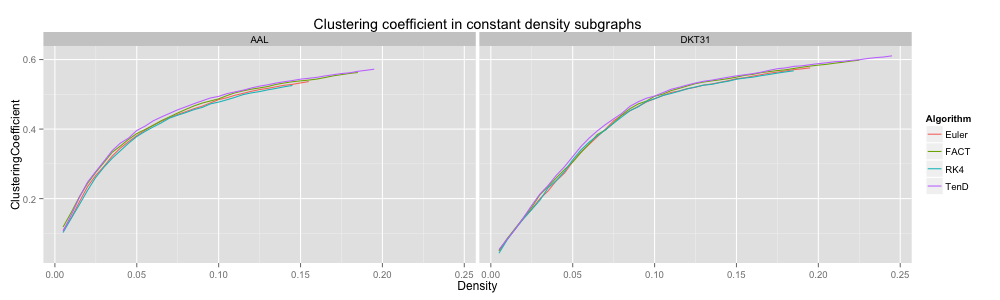
\includegraphics[width=0.5\linewidth]{figures/clust_plot.png}  & 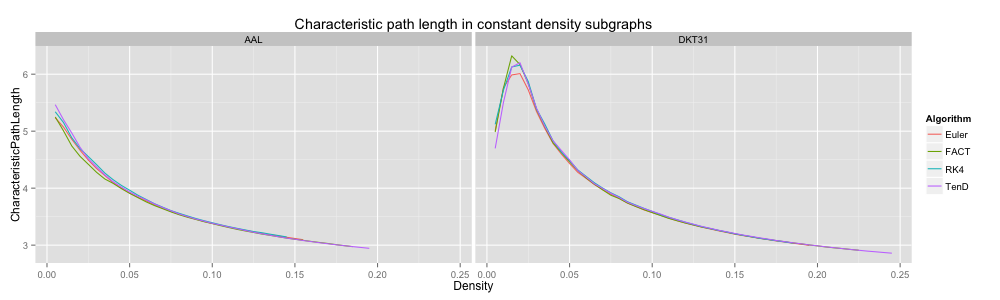
\includegraphics[width=0.5\linewidth]{figures/path_plot.png} \\
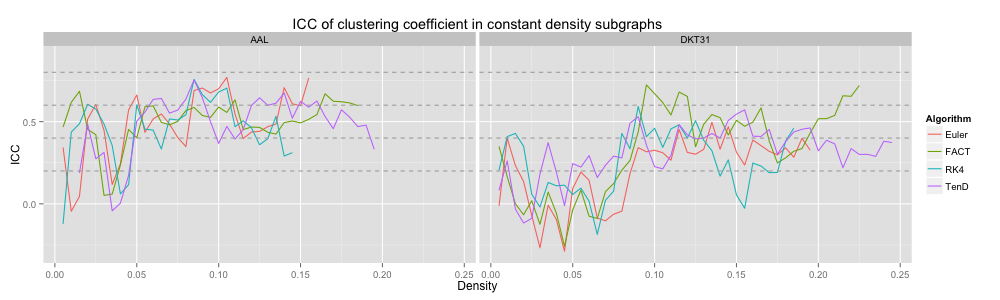
\includegraphics[width=0.5\linewidth]{figures/clust_icc_plot.png} & 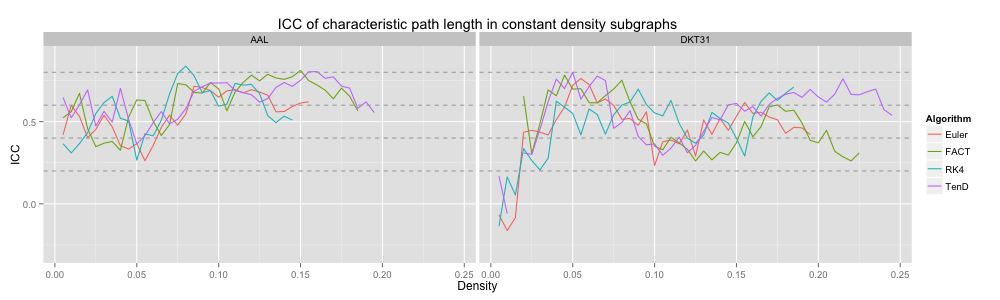
\includegraphics[width=0.5\linewidth]{figures/path_icc_plot.png} \\
A & B \\
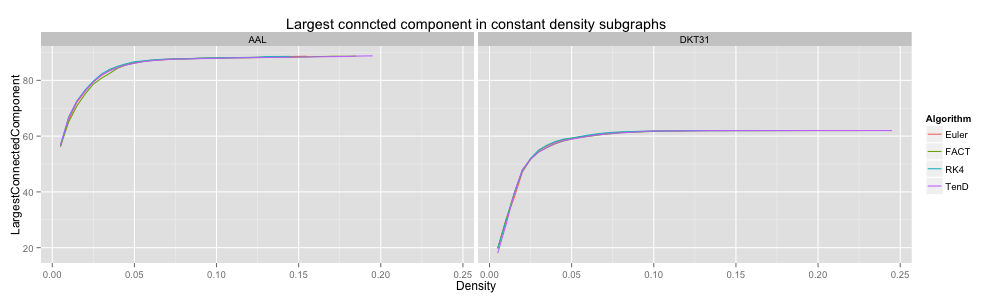
\includegraphics[width=0.5\linewidth]{figures/size_plot.png}  & 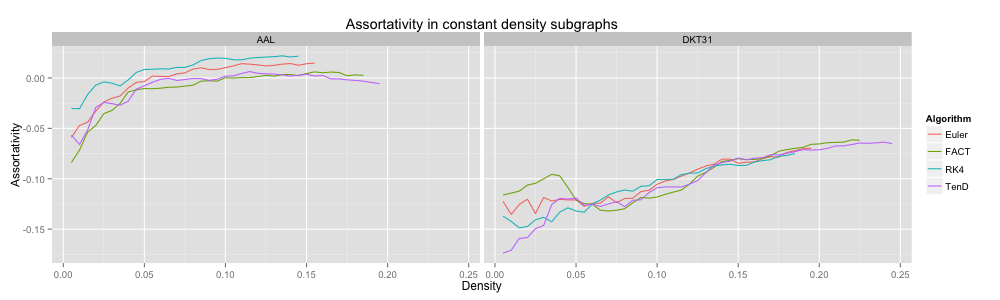
\includegraphics[width=0.5\linewidth]{figures/assort_plot.png} \\
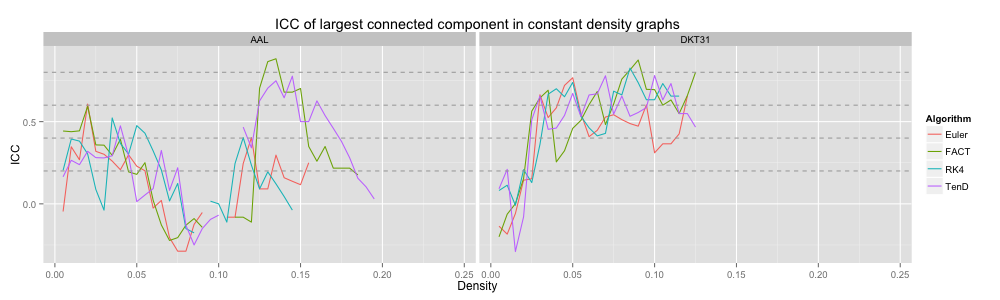
\includegraphics[width=0.5\linewidth]{figures/size_icc_plot.png} & 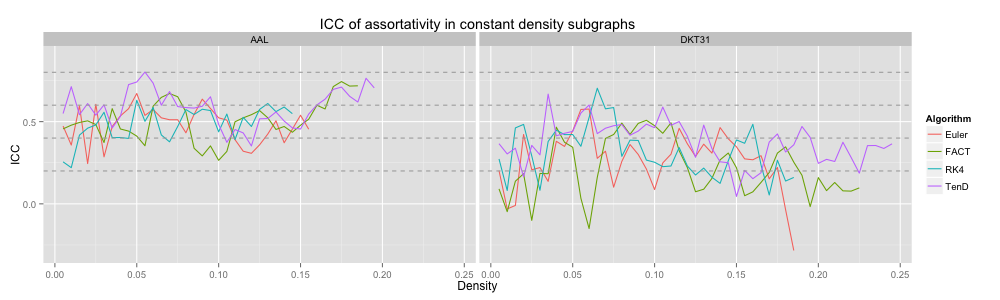
\includegraphics[width=0.5\linewidth]{figures/assort_icc_plot.png} \\
C & D \\
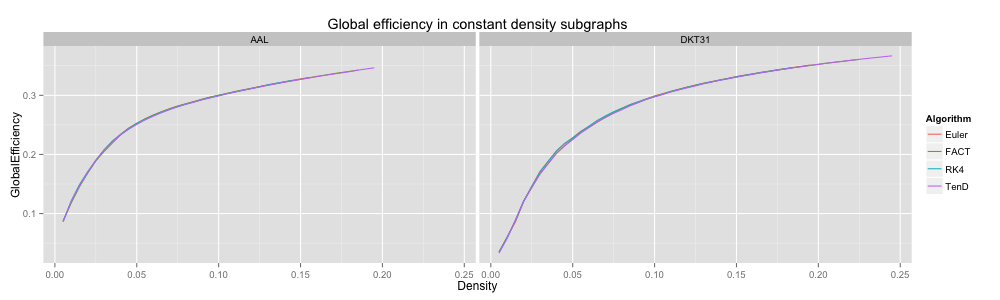
\includegraphics[width=0.5\linewidth]{figures/geff_plot.png}  & 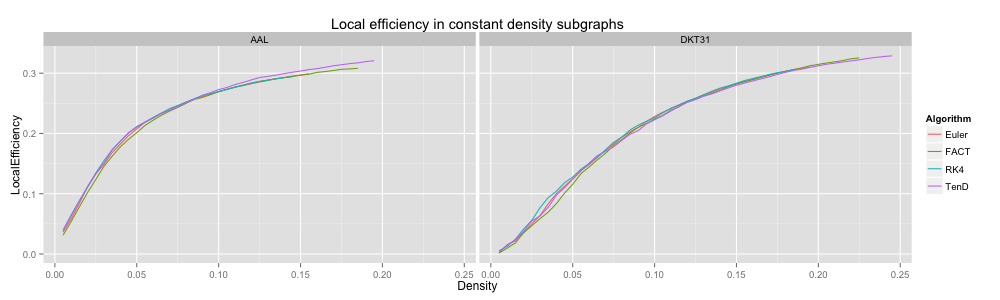
\includegraphics[width=0.5\linewidth]{figures/leff_plot.png} \\
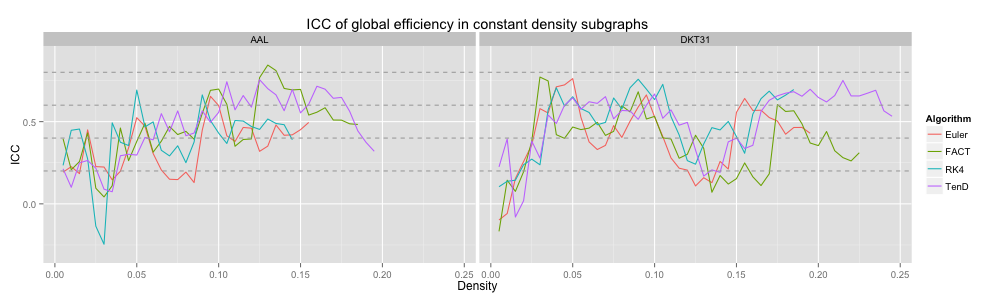
\includegraphics[width=0.5\linewidth]{figures/geff_icc_plot.png} & \includegraphics[width=0.5\linewidth]{figures/leff_icc_plot.png}\\
E & F 
\end{tabular}
\caption{Graph metric vs. graph density plots along with corresponding ICC plots for A) Mean clustering coefficient  B) Characteristic path length C) Largest connected component size D) Assortativity E) Global efficiency and F) Local efficiency}
\label{fig:vsdensity}
\end{center}
\end{figure*}


\begin{table*}[!t]
\processtable{Functional data analysis is used along with permutation
  testing to look for pair-wise differences in graph-metric vs. graph-density curves that result from different
  fiber tracking algorithms and label sets. Only the first time-point for each
  subject is used. For each metric, the upper-triangular values are for p-values for
  the AAL labels while the lower-triangular values were generated with
  the DKT31 label set (* indicated significance).\label{tab:permtesting}}
{\begin{tabular}{l | llll | llll }
\midrule
 & \multicolumn{4}{c}{Clustering Coefficient} &  \multicolumn{4}{c}{Characteristic Path Length} \\ 
\midrule
Euler  &            & 0.2164  & 0.5296    & 0.0346*   &            & 0.2786  & 0.2389    &  0.4728  \\
FACT & 0.6962 &              & 0.0246*  & 0.2822     & 0.9982 &            &  0.0145*   & 0.1235     \\
RK4   & 0.9927 & 0.7958  &               & 0.0049*   & 0.8465 & 0.9199  &                 & 0.3031   \\
TEND & 0.1327 & 0.8858  & 0.2061    &                & 0.4854 & 0.6459  & 0.8234   &    \\ 
\midrule
 & \multicolumn{4}{c}{Connected Component Size} &  \multicolumn{4}{c}{Assortativity} \\ 
\midrule
Euler  &            & 0.3471  & 0.9324    & 0.7556   &            & 0.3680  & 0.3294   &  0.4651  \\
FACT & 0.9447 &              & 0.0468*  & 0.3025     & 0.6361 &            &  0.0270*   & 0.8877     \\
RK4   & 0.9998 &  0.7610  &              & 0.4748   & 0.9326 & 0.3250  &               & 0.0666   \\
TEND & 0.7912 & 0.8336  & 0.7269   &                & 0.8272 & 0.4021  & 0.9895   &    \\ 
\midrule
 & \multicolumn{4}{c}{Global Efficiency} &  \multicolumn{4}{c}{Local efficiency} \\ 
\midrule
Euler  &            & 0.8617  & 0.9861    & 0.7272   &            & 0.4579  & 0.9227   &  0.6065  \\
FACT & 0.8677 &              & 0.6882  & 0.7667     & 0.8794 &            &  0.2486   & 0.1230     \\
RK4   & 0.6295 &  0.9415  &              & 0.8677   & 0.9745 & 0.4413  &               & 0.7557   \\
TEND & 0.9977 & 0.9633  & 0.7438    &                & 0.8752 & 0.7987  & 0.4775   &    \\ 
\midrule
         & Euler    & FACT     & RK4        & TEND       & Euler    & FACT     & RK4        & TEND      \\
\midrule
\end{tabular}}{}
\end{table*}

\subsection{Rich club coefficient over node-degree}
Because the rich club coefficient requires the selection of multiple parameters, we chose to examine how this metric
changes as a function of $k$, the node degree that determines what is considered a 'rich' node. The plots for the
mean graph curves and ICC coefficients are illustrated in figure \ref{fig:richclub}. The results are similar to the examinations
over graph density in that the same shape appears for both label sets, but with a scaling difference and the tracking algorithms
have similar shapes but within the AAL networks, differences were found in the RK4-FACT (p$=$0.0338) and RK4-TEND (p$=$0.0252) 
comparisons. The p-values for all comparisons are listed in table \ref{tab:richp}

\begin{figure}
\begin{center}
\includegraphics[width=0.5\linewidth]{figures/richclub_plot.png} \\
\includegraphics[width=0.5\linewidth]{figures/richclub_icc_plot.png}
\caption{Rich club coefficient was examined over a range of levels, k, and a constant graph density of 0.15}
\label{fig:richclub}
\end{center}
\end{figure}

\begin{table*}[!t]
\processtable{Functional data analysis is used along with permutation
  testing to look for differences in rich club coefficients  
generated from different fiber tracking algorithms. Upper triangular p-values
are for the AAL labels, while lower triangular are for the DTK31 label
set  (* indicated significance).\label{tab:richp}}
{
\begin{tabular}{l | llll }
\midrule
Euler  &            & 0.3359  & 0.6830    & 0.2064   \\
FACT & 0.8944 &              & 0.0338*  & 0.8537     \\
RK4   & 0.9282 & 0.7219   &               & 0.0252*   \\
TEND & 0.7548 & 0.8800  & 0.3360    &                \\             
\midrule
         & Euler    & FACT     & RK4        & TEND        \\
\midrule
\end{tabular}}{}
\end{table*}



%\begin{table}[!t]
%\processtable{Resolution Requirements for the figures\label{Tab:01}}
%{\begin{tabular}{lllll}\toprule
%Image Type & Description & Format & Color Mode & Resolution\\\midrule
%Line Art & An image composed of lines and text,  & TIFF, EPS, JPEG & RGB, Bitmap & 900 - 1200 dpi\\
%          & which does not contain tonal or shaded areas.& & &\\
%         Halftone & A continuous tone photograph, which contains no text. & TIFF, EPS, JPEG & RGB, Grayscale & 300 dpi\\
%Combination & Image contains halftone + text or line art elements. & TIFF, EPS, JPEG & RGB,Grayscale & 600 - 900 dpi\\\botrule
%\end{tabular}}{This is a footnote}
%\end{table}

%\begin{equation}
%\sum x+ y =Z\label{eq:01}
%\end{equation}

%\textbf{Table\ref{Tab:01}} shows the resolution requirements for the figures. The figures must be legible:
%\begin{enumerate}
%\item The smallest visible text is no less than 8 points in height, when viewed at actual size.
%\item Solid lines are not broken up.
%\item Image areas are not pixelated or stair stepped.
%\item Text is legible and of high quality.
%\item Any lines in the graphic are no smaller than 2 points width.
%\end{enumerate}

%\textbf{Figure 2.}{ Enter the caption for your figure here.  Repeat as  necessary for each of your figures.}\label{fig:02}

\section{Discussion}
% Discussion: This section may be divided by subheadings. Discussions
% should cover the key findings of the study: discuss any prior art
% related to the subject so to place the novelty of the discovery in
% the appropriate context; discuss the potential short-comings and
% limitations on their interpretations; discuss their integration into
% the current understanding of the problem and how this advances the
% current views; speculate on the future direction of the research and
% freely postulate theories that could be tested in the future.


%Other modalities, not examined here,
%were also acquired making this data useful for future examinations of
%structure and function.

%No smoothing of data here

%Other DTI scalar metrics, such as RD, or from other modalities such as MTR.
%%
%Did not normalize matrices

\subsection{Network topology}
Although a number of studies have examined the reproducibility of graph metrics on 
structural brain networks derived from DTI-based fiber tractography, there are no known 
papers that focus on the selection of deterministic tracking algorithm. To facilitate later examination of
graph metrics as a function of graph density, we first examined the reliability of identifying
subgraphs by thresholding. Using the dice coefficient as a measure of overlap we demonstrated
that the intra subject agreement was much higher than the inter subject agreement across all tracking algorithms and 
label sets. No significant differences were found for intra-subject comparisons. The inter-subject comparions indicate that 
the TEND method most consistently identifies similar subgraphs at a given density. However, further analysis 
of additional tracking parameters is necessary to determine the full set of conditions under which this result holds.

%However, 
%using the AAL label set we demonstrated differences in inter subject topological similarity between FACT and TEND. 
%This suggests that the TEND algorithm may provide a more reproducible measure of network topology across subjects. 
%This is significant as the AAL labels are prevalent throughout all forms of connectivity studies and the FACT algorithm is the most common choice
%among deterministic tractography methods. 

\subsection{Network summary measures over graph density}
Global and local efficiency are the most robust to choice of fiber tracking algorithm, and have high levels 
of reproducibility across density levels. Assortativity and characteristic path length are highly reproducible across
density levels, but are sensitive to choice of fiber tracking algorithm. In general, the portions of the graph curves
at low density value and less reproducible than the segments at high density.  For many metrics, the graph curves 
strongly converge at high density values suggesting that examining the metrics at those densities may be of 
little use. Examining both the mean graph curves and ICC plots may provide guidance for the range of densities
that should be looked at in a group comparison study. 

\subsection{Rich club coefficient over node-degree}
The examination of rich club coefficient as a function of degree-level demonstrates the use of graph curves over 
a parameter other than graph density. Consistency appears to have a somewhat inverse relationship to the 
coefficient as a function of node degree level. This is a result of the fact that the rich club coefficient values converge
at high and low densities. Here, all graphs were thresholded at the maximum density achievable by all graphs. 
Because network size is held constant here, the average node degree would drop with lowered density, 
and additional work is required to more understand the relationship between graph-density and degree-level that 
would provide the most reproducible results. 

\subsection{Limitations and future directions}
The are a number of methodological limitations to the work presented here. We limited the fiber tracking to deterministic
methods and used constant shared parameters for these methods. The influence of these parameters on individual 
tracking algorithms and the resulting graph metrics demands further exploration. In the choice of anatomical label sets, we
limited the analysis to a set of manually defined labels, and a often used set of template-based labels. In each case we used the labels
'as-is' without upsampling to a higher number of regions. This may reduce the reproducibility of the networks, but provides
more interpretable results if one wishes to examine individual connections or a subset of connections (e.g.\ default mode network)
since the labels have well defined anatomical associations.

The use of a data with relatively low angular resolution and the use
of the diffusion tensor model are both limiting factors in the work presented
here. To some degree, the choice of diffusion model is limited by the
data used here. However, these limitations are representative of a
great deal of existing data sets. Thus, the work presented here
provides insight into the utility of using this data to examine
network-wide structural connectivity properties. Additionally this
work provides a baseline analysis. This allows methods using more sophisticated
techniques, such as diffusion spectrum imaging and it's associated
models, to demonstrate the added value of those methods. Without this
baseline, the added benefit of these more complex techniques is less
clear due to a lack of sufficient context.

An additional limitation of this work is the use of streamline count matrices as the basis for thresholding to create constant
density graphs. Multiple options exist for normalizing the streamline count matrices using the volumes of 
the target cortical regions and/or the average length of the streamlines the connect two regions. The volume based
normalization may accomodate the differences that are seen between graph curves that were generated using 
the different anatomical labels. However, the focus here was on the influence of the fiber tracking and no direct
comparisons were made between graph curves generated from the different label sets. A number of additional options
exist for creating a weighted connectivity matrix including the average FA of fibers that connect two regions. Since the data set
examined also includes magnetization transfer data, the average magnetization transfer ratio along streamlines 
could potentially be useful as it directly related to myelin content in white matter. These issues were beyond the scope 
of the current study but would made for an intriguing extension of the current work. 

The selection of graph metrics for analysis is another limitation of the study. An exhaustive examination of all
possible graph metrics was not feasible so metrics that have been studied previously were chosen to give additional
context to existing work. Many of the metrics examined have alternate formulations for 
weighted graphs. Here, only unweighted graph metrics were examined as they are prevalent in current literature.
 The creation of a testing framework that relies upon a public data set and open-source code
was intended to facilitate the further exploration of the issues listed here.

\subsection{Conclusion}
This study evaluate the reproducibility of graph summary metrics in structural brain networks derived from
DTI based deterministic fiber tractography. Four different fiber tracking algorithms were examined along
with two different anatomical label set. A number of graph metrics were examined by creating graph curves that capture how a metric
changes over a parameter such as graph density. ICC plots were used to evaluate the reproducibility of the metrics and FDA
was used to identify significant differences between graph curves generated using different fiber tracking algorithms.
While differences between the tracking algorithms were not drastic, they were significant in many cases, suggesting
that future studies should give careful consideration to the choice of fiber tracking algorithm based upon the graph
metric that will be analyzed. 


\subsection{Data Sharing}
%Frontiers supports the policy of data sharing, and authors are advised to make freely available any materials and information described in their article, and any data relevant to the article (while not compromising confidentiality in the context of human-subject research) that may be reasonably requested by others for the purpose of academic and non-commercial research. In regards to deposition of data and data sharing through databases, Frontiers urges authors to comply with the current best practices within their discipline.
Free, publicly-available data and software was used throughout. The scripts used to generate the data and figures are available at: \url{https://github.com/jeffduda/StructConnRepro}. This repository contains the configuration file that, when added to ITK, will download and compile Petiole which builds the executables that were used to generate the graph metrics examined in this study. The template with labels is available at \url{http://figshare.com/articles/Kirby_multivariate_template/852989}, the final segmentations used as the target regions for fiber tracking are available at \url{http://figshare.com/articles/MMRR21_DTI_Targets/850369} to provide a convenient starting point for reproducing or extending the methods presented here. 

\section*{Disclosure/Conflict-of-Interest Statement}
%All relationships financial, commercial or otherwise that might be perceived by the academic community as representing a potential conflict of interest must be described. If no such relationship exists, authors will be asked to declare that the research was conducted in the absence of any commercial or financial relationships that could be construed as a potential conflict of interest.
The authors declare that the research was conducted in the absence of any commercial or financial relationships that could be construed as a potential conflict of interest.

%\section*{Acknowledgement}
%Shoutouts to our peeps

%\paragraph{Funding\textcolon} Shoutout to our peep\$

%\section*{Supplemental Data}
%Maybe need this, maybe not

\bibliographystyle{frontiersinSCNS} % for Science articles
%\bibliographystyle{frontiersinMED} % for Medicine articles
\bibliography{priorwork}

%\begin{thebibliography}{}

%\bibitem[Bofelli {et~al}., 2000]{Boffelli03} Bofelli,F., Name2, Name3 (2003) Article title, {\it Journal Name}, 199, 133-154.

%\bibitem[Bag {et~al}., 2001]{Bag01} Bag,M., Name2, Name3 (2001) Article title, {\it Journal Name}, 99, 33-54.

%\end{thebibliography}
\end{document}
